\section{Zielsetzung}
\label{sec:Zielsetzung}

In diesem Versuch sollen Strömungen in Rohren mithilfe des Impuls-Echo-Verfahrens auf ihre charakteristischen Eigenschaften untersucht werden.

\section{Theorie}
\label{sec:Theorie}

Schall mit Frequenzen zwischen $20 \si{\kilo\Hz}$ und $1 \si{\giga\Hz}$ liegt oberhalb der Hörschwelle des Menschen und wird als Ultraschall
bezeichnet.
Die Erzeugung von Ultraschall kann auf verschiedene Arten passieren. In diesem Versuch wird nur der piezo-elektrische Effekt betrachtet.
Piezo-elektrische Kristalle können durch Anregung eines äußeren elektrischen Feldes in Schwingungen versetzt werden.
Die Amplitude der entstehenden Welle und die daraus resultierende Energiedichte kann maximiert werden, indem zwischen Anregungsfrequenz und Eigenfrequenz
des Kristalls Resonanz entsteht.
Außerdem können Piezokristalle als Empfänger genutzt werden, weil sie durch Schallwellen angeregt werden.
Dabei ist Quarz der meist verwendete Piezokristall, weil Quarz gleichbleibende physikalische Eigenschaften besitzt.
Jedoch ist der Piezo-Effekt bei Quarzen relativ gering.\\
Mithilfe von Ultraschall können Informationen über der Aufbau eines Stoffes gewonnen werden.
Als Doppler-Effekt bezeichnet man die Änderung der Frequenz, die durch das Bewegen von Quelle und Empfänger relativ zueinander entsteht.
In dem Fall, in dem sich die Quelle auf den Beobachter zu bewegt wird die Frequenz $\nu_0$ zur höheren Frequenz $\nu_{gr}$ verschoben.
Bewegt sich die Quelle vom Beobachter weg, verschiebt sich $\nu_0$ zur kleineren Frequenz $\nu_{kl}$.
Auch bei einer Bewegung des Beobachters verschiebt sich die Frequenz $\nu_0$.
$\nu_{h}$ ist die höhere Frequenz, zu der sich $\nu_0$ ändert wenn der Beobachter sich auf die Quelle zu bewegt. Bewegt der Beobachter
sich von der Quelle weg, so nimmt $\nu_0$ die niedrigere Frequenz $\nu_{n}$ an.
Die Frequenzen werden durch
\begin{align}
    \nu_{gr/kl}&= \frac{\nu_0}{1 \mp \frac{v}{c}}\label{eqn:nugrkl}\\
    \intertext{für den ruhenden Beobachter und}
    \nu_{h/n}&= \nu_0 \cdot \bigl(1 \pm \frac{v}{c}\bigr)\label{eqn:nuhn}\\
\end{align}
für die ruhende Quelle ausgedrückt.
Der Doppler-Effekt wird im Bereich der Ultraschalltechnologie ausgenutzt, um unter anderem die Geschwindigkeiten von Flüssigkeiten
in Rohren bzw. den Blutstrom in Gefäßen zu messen.
Wenn eine Ultraschallwelle auf ein bewegtes Objekt innerhalb einer Flüssigkeit trifft, so wird die Frequenz $\nu_0$ der Welle um 
\begin{align}
    \Delta \nu &= \nu_0 \frac{v}{c}(\cos{\alpha}+\cos{\beta})\label{eqn:Deltanu1}
\end{align}
gemäß des Doppler-Effekts verschoben. Hierbei sind außer der Geschwindigkeit $v$ des Objektes und der Schallgeschwindigkeit $c$ auch
die Winkel $\alpha$ und $\beta$, zwischen der Geschwindigkeit $v$ und der Wellennormalen der einlaufenden bzw. auslaufenden Welle,
ausschlaggebend.
Wird das Impuls-Echo-Verfahren angewendet, so gilt $\alpha = \beta$ und \autoref{eqn:Deltanu1} reduziert sich auf
\begin{align}
    \Delta \nu &= 2\cdot \nu_0 \frac{v}{c}\cos{\alpha}.\label{eqn:Deltanu}
\end{align}
Die geometrischen Zusammenhänge sind schematisch in \autoref{fig:Abb_1} dargestellt.
\begin{figure}[H]
    \centering
     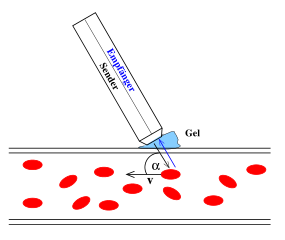
\includegraphics{build/dopplerfluss.png}
    \caption{Schematische Darstellung der Doppler-Sonographie des Blutflusses in einem Gefäß.\cite{VUS3}}
    \label{fig:Abb_1}
\end{figure}

Zur besseren Untersuchung des Flusses in einem Rohr werden Doppler-Prismen verwendet.
So wird die Vermessung der Strömung aus verschiedenen Winkeln unter gleichbleibenden Bedingungen ermöglicht.
Es gilt der Zusammenhang
\begin{align}
    \alpha &= \qty{90}{\degree} - \arcsin{\bigl( \sin{\theta} \cdot \frac{c_L}{c_P}\bigr)},\label{eqn:alpha}
\end{align}
wobei $\theta$ den Prismenwinkel, $\alpha$ den Dopplerwinkel, $c_L$ die Schallgeschwindigkeit der Flüssigkeit und 
$c_P$ die Schallgeschwindigkeit des Prismenmaterials (Acryl) angibt.
Wie in \autoref{fig:Abb_2} zu sehen, ist der Abstand zwischen Sonde und Flüssigkeit
für alle drei Einstellwinkel des Prismas gleich.
\begin{figure}[H]
    \centering
     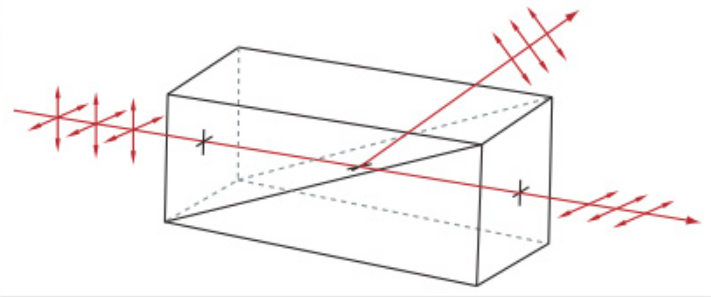
\includegraphics{build/prisma.png}
    \caption{Schematische Darstellung des Dopplerprismas.\cite{VUS3}}
    \label{fig:Abb_2}
\end{figure}
